\chapter{WKB for Eigenvalue Problems}

\paragraph{Example 1:} A Sturm-Liouville problem
\begin{gather*}
	y'' + E Q(x)y = 0  \qquad 0 \leq x \leq \pi   \\
	y(0) = y(\pi) = 0  \qquad Q(x) > 0
\end{gather*}
The ODE has solutions for a discrete set of eigenvalues $E_n$ and corresponding eigenfunctions $y_n$ ($E_n \rightarrow \infty$ as $n \rightarrow \infty$). \\
\ \newline
Interpret $y''$ as curvature (measure of concavity): if $y'' > 0$ it is a parabola opening upwards, etc. Now
\begin{gather*}
	y'' = [-E Q(x)] y 
\end{gather*}
\begin{itemize}
	\item if $E>0$, when $y>0$, $y'' < 0$, i.e. we curve downwards
	\item when $y<0$, $y''>0$ and we curve upwards
\end{itemize}
This implies that we end up with something \emph{sinusoidal}. If the choice of $E$ is not correct, we won't satisfy the right-hand BC. Therefore for a large $n$, we expect $E_n$ to be large which causes the large number of wiggles. This is suggestive of a natural small parameter
\begin{gather*}
	\epsilon^2 = \frac{1}{E} \ll 1
\end{gather*}
This translates our problem to a Schr\"odinger-type equation
\begin{gather*}
	\epsilon^2 y'' = -Q(x) y
\end{gather*}
Using WKB theory (eqn. \ref{eqn:wk18-wkb})
\begin{align*}
	y(x) \sim \frac{1}{[Q(x)]^{1/4}} \left\{ c_1 \sin \left[\frac{1}{\epsilon} \int_{0}^{x} \sqrt{Q(t)} \md t\right] + c_2 \cos \left[\frac{1}{\epsilon} \int_{0}^{x} \sqrt{Q(t)} \md t\right] \right\}
\end{align*}
To satisfy $y(0)=0$, $c_2=0$. To satisfy $y(\pi)=0$, we require
\begin{gather*}
	0 = c_1 \sin \left[\frac{1}{\epsilon}\int_{0}^{\pi} \sqrt{Q(t)}\md t\right]
\end{gather*}
The non-trivial $(c_1 \neq 0)$ solution requires that
\begin{align*}
	\frac{1}{\epsilon} \int_{0}^{\pi} \sqrt{Q(t)\md t} = n\pi, \qquad n = 1,2,3. \dots 
\end{align*}
We cannot have negative $n$ since the LHS is positive. Our eigenvalues are therefore
\begin{align*}
	E_n = \dfrac{n^2 \pi^2}{\left[\int_{0}^{\pi} \sqrt{Q(t)\md t}\right]^2} \qquad \text{as $n \rightarrow \infty$} 
\end{align*}

\paragraph{Example 2:} Two turning points: an example from quantum mechanics
\begin{gather*}
	\epsilon^2 y'' = [V(x)-E]y \\
	y \rightarrow 0 \quad \text{as} \quad |x| \rightarrow \infty
\end{gather*}
\begin{figure}[!h]
	\centering
	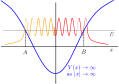
\includegraphics[width=0.5\textwidth]{./plots/pdf/wkb-eigenvalue.pdf}
	\caption{}
	\label{fig:strogatz-wk20}
\end{figure}\\
From Fig. \ref{fig:strogatz-wk20}, and following the example in sec. \ref{sec:turning-points}, we note that to the left of the turning point $B$, the wave solution must match with the wave solution to the right of the turning point at $A$. This is what leads to the quantization. \\
\ \newline
{\bf Schr\"odinger's idea:} Solutions $y(x)$ to this BVP exist only if $E=E_n$, where $E_n$ is an eigenvalue. These are the only allowed energies, i.e. the energy is ``quantized" (whereas classically, any $E$ is allowed as long as $E \geq V_\text{min}$). \\ 
\ \newline
{\bf Strategy:} Using WKB, solve near $A$ and $B$ separately, and then match in the classically permissible region $A<x<B$. \\
\ \newline
\underline{Near $x=B$} \\
\ \newline 
Recall from eqn. \ref{eqn:wk18-wkb} 
\begin{gather*}
	y(x) \sim \frac{c_1}{[V(x)-E]^{1/4}} \exp \left[-\frac{1}{\epsilon} \int_{B}^{x} \sqrt{V(t)-E} \, \md t\right] \qquad x > B
\end{gather*}
Then using the ``connection formula'' (eqn. 10.4.13 in B+O for summary), the matching solution for $A<x<B$ is
\begin{align}
	y(x) \sim \frac{2 c_1}{[E-V(x)]^{1/4}} \sin \left[\frac{1}{\epsilon} \int_{x}^{B} \sqrt{E - V(t)} \md t + \frac{\pi}{4}\right] \label{eqn:wk20-turnpt-B}
\end{align}
\underline{Near $x=A$} 
\begin{gather*}
	y(x) \sim \frac{c_2}{[V(x)-E]^{1/4}} \exp\left[-\frac{1}{\epsilon} \int_{x}^{A} \sqrt{V(t)-E} \, \md t\right] \qquad x<A
\end{gather*}
Similarly, the connection formula through $x=A$ yields
\begin{gather}
	y(x) \sim \frac{2c_2}{[E-V(x)]^{1/4}} \sin \left[\frac{1}{\epsilon} \int_{A}^{x} \sqrt{E-V(t)}\, \md t + \frac{\pi}{4}\right] \label{eqn:wk20-turnpt-A}
\end{gather}
Equations \ref{eqn:wk20-turnpt-B} and \ref{eqn:wk20-turnpt-A} are essentially describing the same behavior and must be identical. This gives us the eigenvalue condition on $E$. The constants $c_1$ and $c_2$ need to be adjusted appropriately, but it is the $x$ dependence through the $\sin[.]$ terms which need careful consideration. 
\begin{align*}
	\sin \left[\frac{1}{\epsilon} \int_{A}^{x} + \frac{\pi}{4}\right] &= \sin \left[\frac{1}{\epsilon}\int_{A}^{B} - \frac{1}{\epsilon}\int_{x}^{B} + \frac{\pi}{4}\right] \\
	&= -\sin \left[\frac{1}{\epsilon}\int_{x}^{B} + \frac{\pi}{4} - \left\{ \frac{1}{\epsilon}\int_{A}^{B} + \frac{\pi}{2} \right\} \right] \\
	&= -\sin \left[\frac{1}{\epsilon} \int_{x}^{B} + \frac{\pi}{4}\right] \cos K + \cos\left[\frac{1}{\epsilon} \int_{x}^{B} + \frac{\pi}{4}\right] \sin K
\end{align*}
where
\begin{gather*}
	K = \frac{1}{\epsilon} \int_{A}^{B} + \frac{\pi}{2}
\end{gather*}
is a constant (no $x$ dependence). Now \underline{iff}
\begin{gather*}
	\sin K = 0 \\
	\implies K = n\pi, \qquad n=0,\pm 1,\pm 2, \dots 
\end{gather*}
would the $x$ dependence match. Therefore
\begin{align*}
	\frac{1}{\epsilon} \int_{A}^{B} \sqrt{E_n-V(t)} \, \md t &= \left(n-\frac{1}{2}\right)\pi, \qquad n=1,2,3 \dots \\
	&= \left(n+\frac{1}{2}\right)\pi, \qquad n = 0,1,2, \dots 
\end{align*}
since the integrand $>0$ on $A<x<B$. The formula works (asymptotically) if either $\epsilon \ll 1$, with $E$ fixed, \underline{or}, $n\gg 1$ and $E_n \gg 1$ with $\epsilon$ fixed (B+O, p.521). This can be understood from the rescaling of the equation
\begin{gather*}
	\tilde{\epsilon}^2 = \frac{\epsilon^2}{E} \qquad Q(x) = \frac{V(x)-E}{E}
\end{gather*}


\paragraph{Example 3:} The quantum-harmonic oscillator
\begin{gather*}
	V(x) = x^2
\end{gather*}
Here $E=V(x)$ at $x = \pm \sqrt{E}$. Here take $\epsilon=1$ and $n\gg 1$. The eigencondition is
\begin{align*}
	\int_{-\sqrt{E}}^{+\sqrt{E}} \sqrt{E - x^2} = \left(n+ \frac{1}{2}\right) \pi 
\end{align*} 
Let $x=u\sqrt{E}$ 
\begin{gather*}
	E \underbrace{\int_{-1}^{1} \sqrt{1 - u^2} \, \md u}_{\pi/2} = \left(n+\frac{1}{2}\right) \pi \\
	\implies E_n = 2n+1, \qquad n=0,1,2,\dots 
\end{gather*}
Here the integral is simply the area of a unit semi-circle in the $u-v$ plane, such that $u^2+v^2=1$. Now WKB tells us that this is valid for $n\gg 1$, but this is in fact exact for all $n$ (can be shown). In physics, the \emph{time-independent 1D Schr\"odinger} equation reads
\begin{gather*}
	-\frac{\hbar^2}{2m} \psi '' + V(x) \psi = E \psi 
\end{gather*}
where $\hbar$ is the Planck's constant divided by $2\pi$. The energy levels come out to be
\begin{gather*}
	E_n = \left(2n+1\right) \frac{\hbar \omega}{2} 
\end{gather*}


